%%
% 第二章：系统设计与实现
%%

\chapter{系统设计与实现}
\label{chap:design}

\section{系统架构}

PathTracer系统采用模块化设计，由以下核心组件构成：

\begin{figure}[htbp]
    \centering
    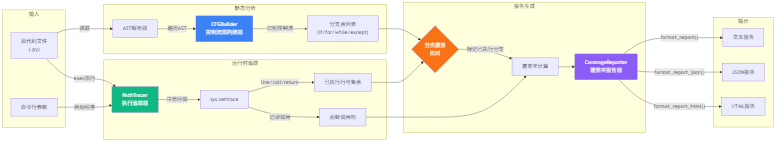
\includegraphics[width=0.95\textwidth]{figures/pathtracer-architecture.png}
    \caption{PathTracer系统架构图}
    \label{fig:architecture}
\end{figure}

\subsection{模块划分}

系统主要包含以下模块：

\begin{table}[htbp]
    \centering
    \caption{模块职责划分}
    \label{tab:modules}
    \begin{tabular}{llp{6cm}}
        \toprule
        \textbf{模块} & \textbf{文件} & \textbf{核心职责} \\
        \midrule
        数据模型 & models.py & 定义分支类型枚举、代码分支、函数调用、执行路径、覆盖率报告等数据结构 \\
        运行时追踪 & tracer.py & 使用\texttt{sys.settrace}追踪程序执行，记录行号和函数调用 \\
        控制流分析 & cfg\_builder.py & 使用AST静态分析识别源代码中的所有分支点 \\
        报告生成 & reporter.py & 对比静态分支与执行路径，计算覆盖率，生成多格式报告 \\
        命令行接口 & cli.py & 解析命令行参数，协调各模块工作流程 \\
        \bottomrule
    \end{tabular}
\end{table}

\section{核心数据模型}

\subsection{分支类型枚举}

定义了程序中可能出现的控制流分支类型：

\begin{lstlisting}[language=Python, caption=分支类型枚举定义]
class BranchType(Enum):
    """控制流分支类型枚举"""
    SEQUENTIAL = "sequential"  # 顺序执行
    IF = "if"                  # if条件语句
    ELSE = "else"              # else分支
    ELIF = "elif"              # elif分支
    FOR = "for"                # for循环
    WHILE = "while"            # while循环
    TRY = "try"                # try异常捕获块
    EXCEPT = "except"          # except异常处理块
\end{lstlisting}

\subsection{代码分支数据类}

\texttt{CodeBranch}表示源代码中的一个分支点：

\begin{lstlisting}[language=Python, caption=CodeBranch数据类]
@dataclass
class CodeBranch:
    """表示代码中的一个分支点"""
    file_path: str           # 源文件路径
    line_no: int             # 分支起始行号
    branch_type: BranchType  # 分支类型
    end_line: int = 0        # 分支结束行号
    is_executed: bool = False # 运行时是否被执行
\end{lstlisting}

\subsection{函数调用记录类}

\texttt{FunctionCall}记录函数调用信息，支持嵌套调用树：

\begin{lstlisting}[language=Python, caption=FunctionCall数据类]
@dataclass
class FunctionCall:
    """记录函数调用信息"""
    function_name: str              # 函数名
    file_path: str                  # 所在文件
    line_no: int                    # 调用行号
    call_depth: int                 # 调用深度（0为顶层）
    arguments: Dict[str, str]       # 参数名到值的映射
    return_value: Optional[str]     # 返回值（repr后的字符串）
    children: List['FunctionCall']  # 子调用列表
\end{lstlisting}

\subsection{覆盖率报告类}

\texttt{CoverageReport}汇总分析结果：

\begin{lstlisting}[language=Python, caption=CoverageReport数据类]
@dataclass
class CoverageReport:
    """覆盖率分析报告"""
    total_branches: int = 0           # 总分支数
    executed_branches: int = 0        # 已执行分支数
    branches_by_type: Dict[BranchType, int]  # 按类型统计
    coverage_percentage: float = 0.0  # 覆盖率百分比
    file_reports: Dict[str, ExecutionPath]   # 各文件详细报告
\end{lstlisting}

\section{运行时追踪器实现}

\subsection{sys.settrace机制原理}

Python的\texttt{sys.settrace}函数允许注册一个全局追踪回调。当程序执行时，解释器会在每个"事件"发生时调用该回调：

\begin{table}[htbp]
    \centering
    \caption{追踪事件类型}
    \label{tab:events}
    \begin{tabular}{lp{8cm}}
        \toprule
        \textbf{事件} & \textbf{触发时机} \\
        \midrule
        'call' & 函数被调用时（进入函数体前） \\
        'line' & 即将执行新的一行代码时 \\
        'return' & 函数即将返回时（arg为返回值） \\
        'exception' & 发生异常时（arg为异常元组） \\
        \bottomrule
    \end{tabular}
\end{table}

\subsection{追踪回调函数核心实现}

\begin{lstlisting}[language=Python, caption=追踪回调函数实现]
def _trace_callback(self, frame, event: str, arg):
    """内部追踪回调函数

    Args:
        frame: 当前栈帧对象，包含代码对象、局部变量等
        event: 事件类型 ('call', 'line', 'return', 'exception')
        arg: 事件相关参数 (return时为返回值，exception时为异常信息)

    Returns:
        返回自身以继续追踪，或None停止追踪
    """
    if not self._target_file:
        return None

    code = frame.f_code
    # 只追踪目标文件
    if not code.co_filename.endswith(self._target_file):
        return self._trace_callback

    if event == 'line':
        # 记录执行的行号
        line_no = frame.f_lineno
        self.execution_paths[self._target_file] \
            .executed_lines.add(line_no)

    elif event == 'call':
        # 提取函数名和参数
        func_name = code.co_name
        args = self._extract_arguments(frame, code)
        # 构建函数调用对象
        call_depth = len(self._call_stack)
        func_call = FunctionCall(
            function_name=func_name,
            file_path=code.co_filename,
            line_no=frame.f_lineno,
            call_depth=call_depth,
            arguments=args
        )
        # 添加到调用树
        if self._call_stack:
            self._call_stack[-1].children.append(func_call)
        else:
            self.function_calls.append(func_call)
        self._call_stack.append(func_call)

    elif event == 'return':
        # 弹出调用栈，记录返回值
        if self._call_stack:
            func_call = self._call_stack.pop()
            if arg is not None:
                func_call.return_value = repr(arg)

    return self._trace_callback
\end{lstlisting}

\subsection{参数提取实现}

\begin{lstlisting}[language=Python, caption=函数参数提取]
def _extract_arguments(self, frame, code) -> Dict[str, str]:
    """从栈帧中提取函数参数

    利用code对象获取参数名列表，从frame.f_locals获取参数值
    """
    args = {}
    try:
        arg_count = code.co_argcount
        arg_names = code.co_varnames[:arg_count]
        for arg_name in arg_names:
            if arg_name in frame.f_locals:
                try:
                    args[arg_name] = repr(frame.f_locals[arg_name])
                except Exception:
                    args[arg_name] = '<unable to repr>'
    except Exception:
        pass
    return args
\end{lstlisting}

\subsection{上下文管理器接口}

使用Python的上下文管理器协议简化追踪的启动和停止：

\begin{lstlisting}[language=Python, caption=上下文管理器实现]
def __enter__(self):
    """进入上下文：保存原追踪函数，启动追踪"""
    self._original_trace = sys.gettrace()
    sys.settrace(self._trace_callback)
    return self

def __exit__(self, exc_type, exc_val, exc_tb):
    """退出上下文：恢复原追踪函数"""
    sys.settrace(self._original_trace)
    return False  # 不抑制异常
\end{lstlisting}

使用示例：
\begin{lstlisting}[language=Python]
tracer = PathTracer().trace_file("target.py")
with tracer:
    # 在此执行目标代码
    result = target_function()
# 退出with块后自动停止追踪
\end{lstlisting}

\section{控制流图构建器}

\subsection{AST遍历原理}

Python的\texttt{ast}模块可以将源代码解析为抽象语法树。通过遍历AST，可以识别所有控制流节点：

\begin{lstlisting}[language=Python, caption=AST遍历构建CFG]
def build_from_file(self, file_path: str) -> List[CodeBranch]:
    """从Python文件构建控制流图

    Args:
        file_path: Python源文件路径

    Returns:
        识别到的所有分支点列表
    """
    with open(file_path, 'r', encoding='utf-8') as f:
        source = f.read()

    # 解析源代码为AST
    tree = ast.parse(source, filename=file_path)
    self.branches = []

    # 遍历AST，提取控制流节点
    for node in ast.walk(tree):
        branch = self._extract_branch(file_path, node)
        if branch:
            self.branches.append(branch)

    return self.branches
\end{lstlisting}

\subsection{分支节点识别}

\begin{lstlisting}[language=Python, caption=分支节点识别逻辑]
def _extract_branch(self, file_path: str, node: ast.AST):
    """从AST节点提取分支信息

    识别if/for/while/except等控制流结构
    """
    # if条件语句
    if isinstance(node, ast.If):
        return CodeBranch(
            file_path=file_path,
            line_no=node.lineno,
            branch_type=BranchType.IF,
            end_line=self._get_end_line(node)
        )

    # for循环
    elif isinstance(node, ast.For):
        return CodeBranch(
            file_path=file_path,
            line_no=node.lineno,
            branch_type=BranchType.FOR,
            end_line=self._get_end_line(node)
        )

    # while循环
    elif isinstance(node, ast.While):
        return CodeBranch(
            file_path=file_path,
            line_no=node.lineno,
            branch_type=BranchType.WHILE,
            end_line=self._get_end_line(node)
        )

    # except异常处理器
    elif isinstance(node, ast.ExceptHandler):
        return CodeBranch(
            file_path=file_path,
            line_no=node.lineno,
            branch_type=BranchType.EXCEPT,
            end_line=self._get_end_line(node)
        )

    return None
\end{lstlisting}

\subsection{结束行号计算}

\begin{lstlisting}[language=Python, caption=结束行号计算]
def _get_end_line(self, node: ast.AST) -> int:
    """获取代码块的结束行号

    优先使用Python 3.8+的end_lineno属性，
    否则递归计算body中最大的行号
    """
    # Python 3.8+ 提供end_lineno属性
    if hasattr(node, 'end_lineno') and node.end_lineno is not None:
        return node.end_lineno

    # 递归计算body中的最大行号
    if hasattr(node, 'body') and node.body:
        return max(self._get_end_line(n) for n in node.body)

    return getattr(node, 'lineno', 0)
\end{lstlisting}

\section{报告生成器}

\subsection{覆盖率计算核心逻辑}

\begin{lstlisting}[language=Python, caption=覆盖率计算实现]
def analyze(self, file_path: str, tracer: PathTracer) -> CoverageReport:
    """分析覆盖率

    Args:
        file_path: 要分析的文件路径
        tracer: 已执行追踪的PathTracer实例

    Returns:
        CoverageReport: 覆盖率报告对象
    """
    # 1. 静态分析：获取所有分支点
    all_branches = self.cfg_builder.build_from_file(file_path)

    # 2. 动态追踪：获取已执行行号
    executed_lines = tracer.get_executed_lines(file_path)

    # 3. 标记已执行的分支
    for branch in all_branches:
        if branch.line_no in executed_lines:
            branch.is_executed = True

    # 4. 计算统计指标
    total = len(all_branches)
    executed = sum(1 for b in all_branches if b.is_executed)

    # 5. 按类型统计
    by_type: Dict[BranchType, int] = {}
    for branch_type in BranchType:
        type_branches = [b for b in all_branches
                        if b.branch_type == branch_type]
        by_type[branch_type] = len(type_branches)

    # 6. 构建报告对象
    return CoverageReport(
        total_branches=total,
        executed_branches=executed,
        branches_by_type=by_type,
        coverage_percentage=(executed / total * 100) if total > 0 else 0.0,
        file_reports={file_path: ExecutionPath(...)}
    )
\end{lstlisting}

\subsection{覆盖率计算公式}

覆盖率计算公式：

\begin{equation}
    \label{eq:coverage}
    \text{Coverage} = \frac{N_{executed}}{N_{total}} \times 100\%
\end{equation}

其中：
\begin{itemize}
    \item $N_{total}$：静态分析识别的总分支数
    \item $N_{executed}$：运行时实际执行的分支数
\end{itemize}

\subsection{多格式报告输出}

\begin{table}[htbp]
    \centering
    \caption{报告输出格式}
    \label{tab:format}
    \begin{tabular}{llp{5cm}}
        \toprule
        \textbf{格式} & \textbf{方法} & \textbf{特点} \\
        \midrule
        文本 & format\_report() & 纯文本，适合控制台输出 \\
        JSON & format\_report\_json() & 结构化数据，便于程序处理 \\
        HTML & format\_report\_html() & 带语法高亮，适合可视化查看 \\
        \bottomrule
    \end{tabular}
\end{table}

\section{HTML报告生成}

\subsection{HTML报告结构}

HTML报告包含以下部分：

\begin{enumerate}
    \item \textbf{摘要卡片}：覆盖率百分比、总分支数、已执行分支数
    \item \textbf{分支类型统计}：按if/for/while/except分类的统计
    \item \textbf{源代码展示}：带行号和执行状态高亮的代码
    \item \textbf{函数调用树}：嵌套展示函数调用关系
\end{enumerate}

\subsection{执行状态视觉区分}

\begin{table}[htbp]
    \centering
    \caption{代码行状态样式}
    \label{tab:styles}
    \begin{tabular}{lll}
        \toprule
        \textbf{状态} & \textbf{背景色} & \textbf{边框} \\
        \midrule
        已执行 & 绿色半透明 (\texttt{rgba(40,167,69,0.15)}) & 绿色左边框 \\
        未执行 & 红色半透明 (\texttt{rgba(220,53,69,0.15)}) & 红色左边框 \\
        \bottomrule
    \end{tabular}
\end{table}

\section{本章小结}

本章详细介绍了PathTracer系统的设计与实现：

\begin{enumerate}
    \item \textbf{数据模型}：使用Python dataclass定义分支类型、代码分支、函数调用、覆盖率报告等核心数据结构
    \item \textbf{运行时追踪}：基于\texttt{sys.settrace}实现，支持line/call/return事件追踪
    \item \textbf{静态分析}：基于AST遍历识别if/for/while/except控制流结构
    \item \textbf{报告生成}：支持文本/JSON/HTML三种输出格式
\end{enumerate}

整个系统仅依赖Python标准库，无需安装第三方依赖，具有良好的可移植性。
